\section{Hướng dẫn build phần mềm}
Để có thể chạy game trên Windows, trước tiên ta cần phải đặt Python thông qua phần mềm Anaconda. Chi tiết cài đặt có hướng dẫn ở trang chủ: \url{https://docs.conda.io/projects/conda/en/latest/user-guide/install/windows.html}.
\begin{figure}[H]
\centering{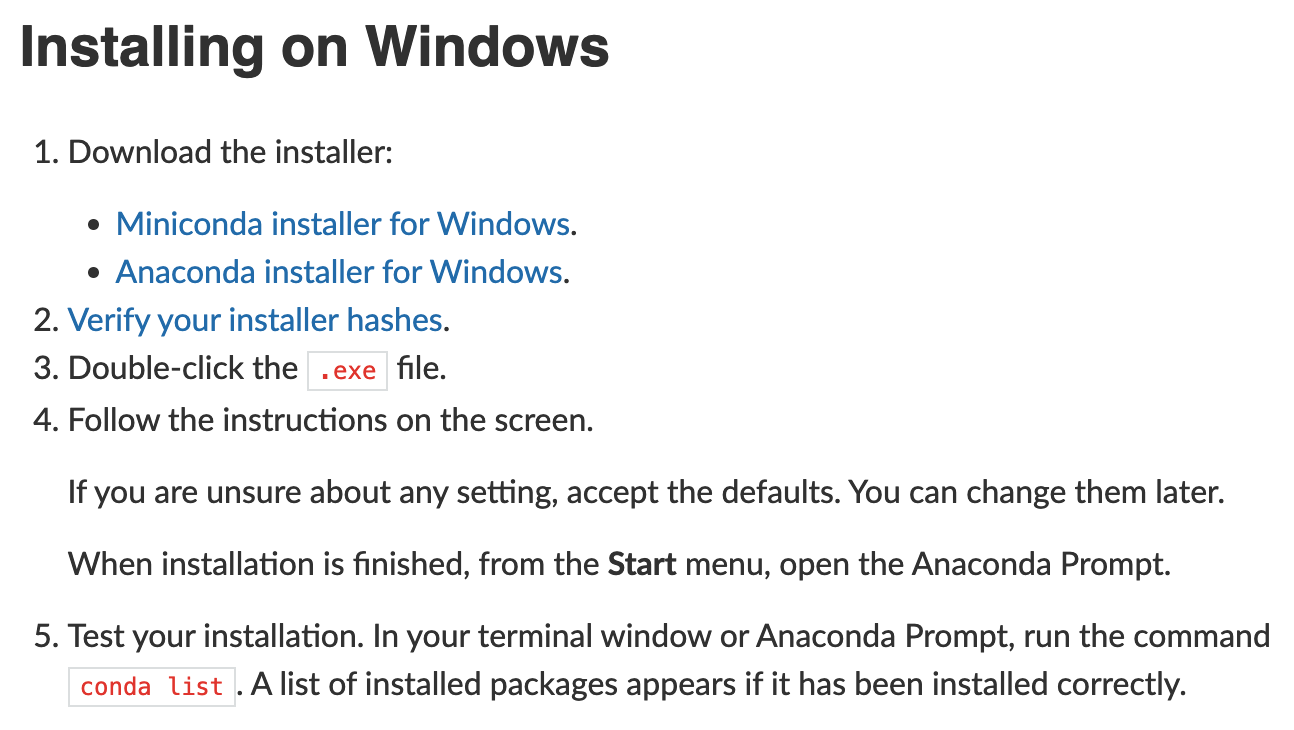
\includegraphics[scale=0.4]{images/anaconda.png}}
\caption{Hướng dẫn cài đặt Anaconda}
\end{figure}
Sau khi cài đặt Anaconda thành công, ta vào thư mục \textbf{source-code}. Gõ cmd ở đường dẫn của thư mục và nhấn \textbf{Enter} để mở cửa sổ \textbf{cmd} với thư mục hiện tại.
\begin{figure}[H]
\centering{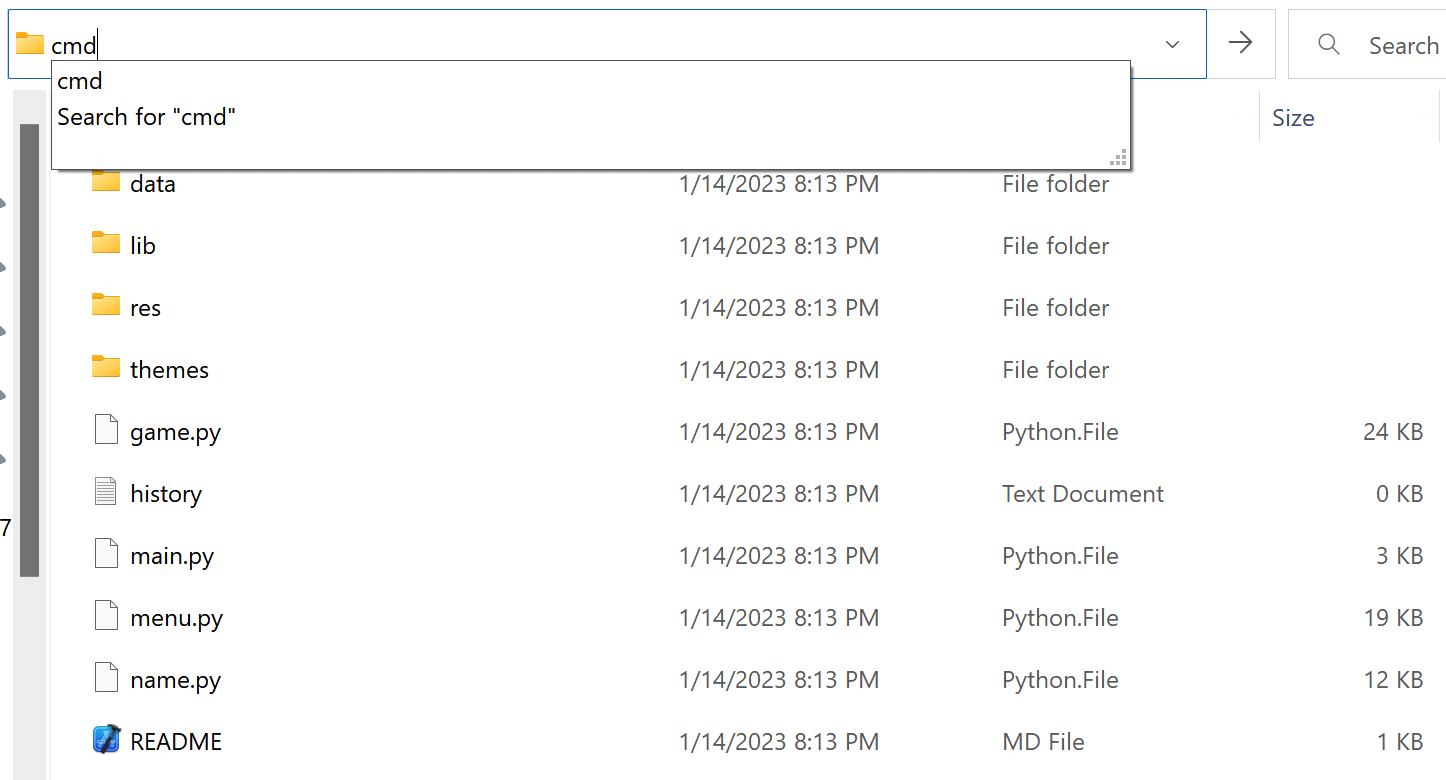
\includegraphics[scale=0.4]{images/source-code.png}}
\caption{Thư mục source-code}
\end{figure}
Lần lượt nhập các lệnh sau để khởi tạo môi trường Python riêng cho game:
\begin{lstlisting}https://www.overleaf.com/project/63c3a1b0d79b43b0c5a021fb
conda create -n caro_A1 python=3.6.3 -y
conda activate caro_A1
\end{lstlisting}

Sau đó nhập các lệnh sau để cài đặt các thư viện cần thiết
\begin{lstlisting}https://www.overleaf.com/project/63c3a1b0d79b43b0c5a021fb
pip install pygame
pip install pygame_gui
\end{lstlisting}

Cuối cùng ta thực hiện lệnh sau để chạy chương trình:
\begin{lstlisting}https://www.overleaf.com/project/63c3a1b0d79b43b0c5a021fb
python main.py
\end{lstlisting}